\documentclass[PianoDiQualifica.tex]{subfiles}

\begin{document}

\chapter{Resoconto attività di verifica}

\section{Revisione dei Requisiti}
\subsection{Qualità di processo}

In questa sezione del documento vengono analizzati i processi, gli esiti delle attività di \citGloss{verifica} svolte su tutti i documenti che vengono consegnati nelle revisioni di progetto e sul prodotto software in sviluppo.

\subsubsection{Metriche processi}
\begin{table}[H]
	\begin{center}
		\begin{tabu} to \textwidth {
				>{\centering}m{0.13\linewidth}
				>{\centering}m{0.15\linewidth}
				>{\centering}m{0.5\linewidth} 
				>{\centering}m{0.12\linewidth} 				
			}
			\tableHeaderStyle
			\textbf{ID} & \textbf{Valore ottenuto} & \textbf{Commento} & \textbf{Esito} \\
			\textbf{MPS001} & -1 giorno & Un giorno di lavoro aggiuntivo siccome l' attività di documentazione e analisi \citGloss{requisiti} è terminata l'11 Gennaio dopo incontro & Ottimo \\
			\textbf{MPS002} & -9,92\% & Dovuto a maggior \citGloss{verifica} e analisi rispetto pianificazione & Accettato \\
			\textbf{MPS007} & 1 & Dovuto ad aggiornamento servizi in seguito a dichiarazioni attacchi informatici Spectre e Meltdown: \nURI{https://goo.gl/pTdGGY}  & Ottimo \\
			\textbf{MPS008} & 0 & Attività di lavoro non ha avuto eventi imprevisti o manifestazione nuovi rischi & Ottimo \\
			
		\end{tabu}
		\caption{Resoconto delle misurazioni delle metriche di processo}
		\vspace{-1em}
	\end{center}
\end{table}
\subsubsection{Maturità processi ISO 15504}
\begin{table}[H]
	\begin{center}
		\begin{tabu} to \textwidth {
				>{\centering}m{0.24\linewidth}
				>{\centering}m{0.33\linewidth}
				>{\centering}m{0.43\linewidth} 
			}
			\tableHeaderStyle
			\textbf{ID} & \textbf{Livello maturità: 1 a 5} & \textbf{Commento} \\
			\textbf{PROC001} & 2 & Gestito tramite software, come \citGloss{Asana}, ha permesso di ottenere risultati positivi nella pianificazione  \\ 
			\textbf{PROC002} & 0 & Sarà istanziato dalla consegna documenti revisione requisiti per creazione \citGloss{proof of concept} \\ 
			
			\textbf{PROC003} & 2 & Completamente automatico ma con calcolo finale manuale da automatizzare \\ 
		\end{tabu}
		\caption{Resoconto del livello maturità processi}
		\vspace{-1em}
	\end{center}
\end{table}

\subsection{Qualità di prodotto}
In questa fase del progetto le uniche metriche di prodotto istanziate sono quelle riguardanti i documenti.
\subsubsection{Errori ortografici}
Tutti i documenti, dopo l'attento lavoro dei verificatori e il feedback positivo rilasciato dallo strumento di controllo ortografico dell'ambiente \citGloss{TexStudio}, risultano privi di errori ortografici, raggiungendo il valore accettabile e ottimale della metrica \textlink{MPDD003TAB}{MPDD003}{\textbf{MPDD003 Errori ortografici}}.

\subsubsection{Indice di Gulpease}
Grazie ad alcuni script automatici è stato possibile istanziare la metrica \textlink{MPDD001TAB}{MPDD001}{\textbf{MPDD001 Indice di Gulpease}} in modo coerente e ripetibile.\\
L'esecuzione degli script ha rivelato l'ottimo lavoro dei redattori, ottenendo valori nei range di accettazione per 2 documenti e valori nel range ottimale per 8 documenti, su un totale di 10.\\
Nella tabella sottostante è mostrato il dettaglio dei risultati ottenuti.
\begin{table}[H]
	\begin{center}
		\begin{tabu} to \textwidth {
				>{\centering}m{0.34\linewidth}
				>{\centering}m{0.33\linewidth}
				>{\centering}m{0.33\linewidth} 
			}
			\tableHeaderStyle
			\textbf{Nome documento} & \textbf{Indice di Gulpease} & \textbf{Esito} \\
			\textbf{Piano di Progetto} & 62.09 & Ottimo \\
			\textbf{Piano di Qualifica} & 52.89 & Accettato \\
			\textbf{Norme di Progetto} & 60.17 & Ottimo \\
			\textbf{Analisi dei Requisiti} & 91.08 & Ottimo \\
			\textbf{Studio di Fattibilità} & 58.72 & Accettato \\
			\textbf{Lettera di Presentazione} & 94.62 & Ottimo \\
			\textbf{VER-2017-11-13} & 67.55 & Ottimo \\
			\textbf{VER-2017-11-22} & 63.78 & Ottimo \\
			\textbf{VER-2017-12-08} & 63.04 & Ottimo \\
			\textbf{VER-2018-01-09} & 69.79 & Ottimo \\
			
		\end{tabu}
		\caption{Resoconto delle misurazioni sulla metrica MPDD001 - Indice di Gulpease}
		\vspace{-1em}
	\end{center}
\end{table}

\subsubsection{Formula di Flesch}
Non essendo ancora presenti documenti redatti in lingua inglese, non c'è stata ragione di istanziare questa metrica.
	
\subsection{Conclusioni}
Il gruppo ha utilizzato complessivamente quasi 24 ore in più rispetto alla pianificazione di inizio periodo, con un MPS002 (Budget Variance) di -9,92\% con rispettivo aumento di 375 euro.\\
Tale passivo non andrà influenzare il costo del progetto come spiegato nel Consuntivo del \pdp{}.
Inoltre l'investimento di un numero maggiore di ore è stato dovuto all'attualizzazione di processi con il maggior numero possibile di procedure e/o automazioni per diminuire il carico di lavoro futuro nello sviluppo della documentazione.

	
\section{Revisione di Progettazione}
	
\subsection{Qualità di processo}
In questa sezione del documento vengono analizzati i processi, gli esiti delle attività di \citGloss{verifica} svolte su tutti i documenti che vengono consegnati nelle revisioni di progetto e sul prodotto software in sviluppo.

\subsubsection{Metriche processi}

\textbf{MPS001 Schedule Variance}
\begin{figure}[htb]
	\centering
	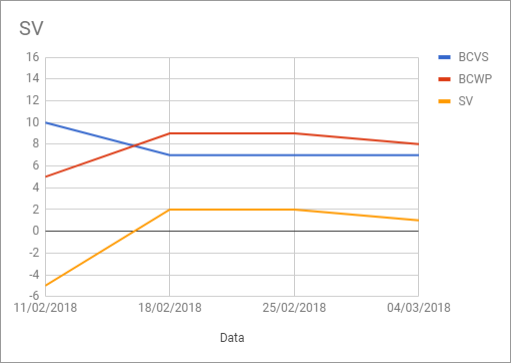
\includegraphics[width=0.5\linewidth]{RP/SV}
	\caption{MPS001}
	\label{fig:processi}
\end{figure}

\textbf{MPS002 Budget Variance}
\begin{figure}[htb]
	\centering
	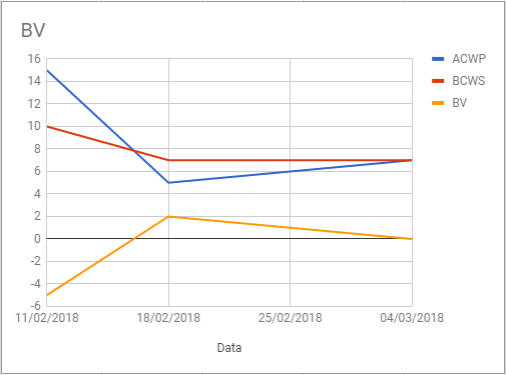
\includegraphics[width=0.5\linewidth]{RP/BV}
	\caption{MPS002}
	\label{fig:processi}
\end{figure}


\newpage
\textbf{Coverage}
\\
	\textbf{MPS003, MPS004, MPS005 e MPS006}
\\
\textbf{Attenzione:} pur non essendo ancora impegnati nella progettazione e realizzazione del prodotto ma solo di un Proof of concept il gruppo ha voluto imparare ed utilizzare gli strumenti legati alla generazione del coverage.
\begin{figure}[htb]
	\centering
	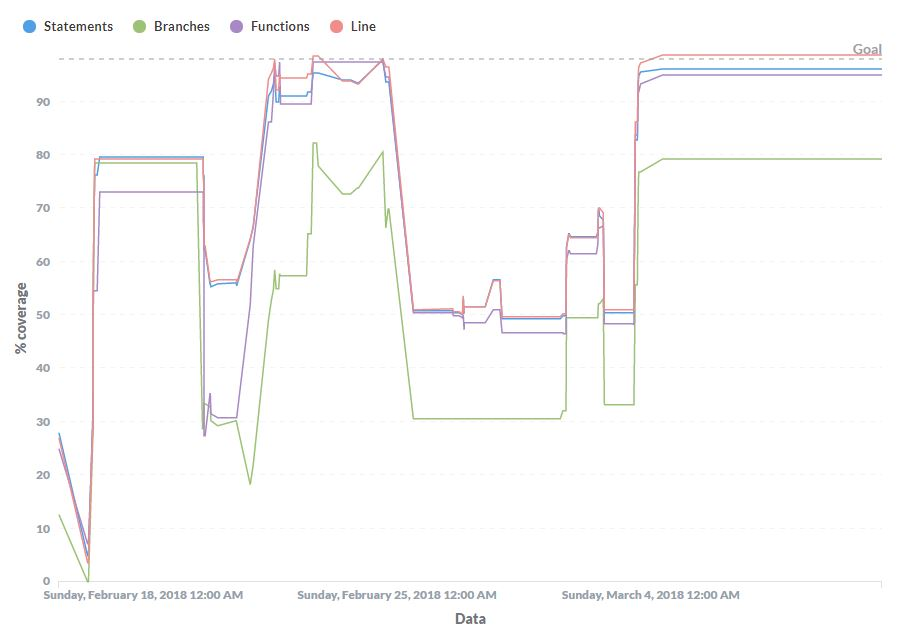
\includegraphics[width=1\linewidth]{RP/coverage}
	\caption{Andamento generale coverage}
	\label{fig:processi}
\end{figure}
\newpage


\textbf{MPS007 Indisponibilità servizi esterni}\\
Misurazione periodo RP: \textbf{1}
\begin{figure}[htb]
	\centering
	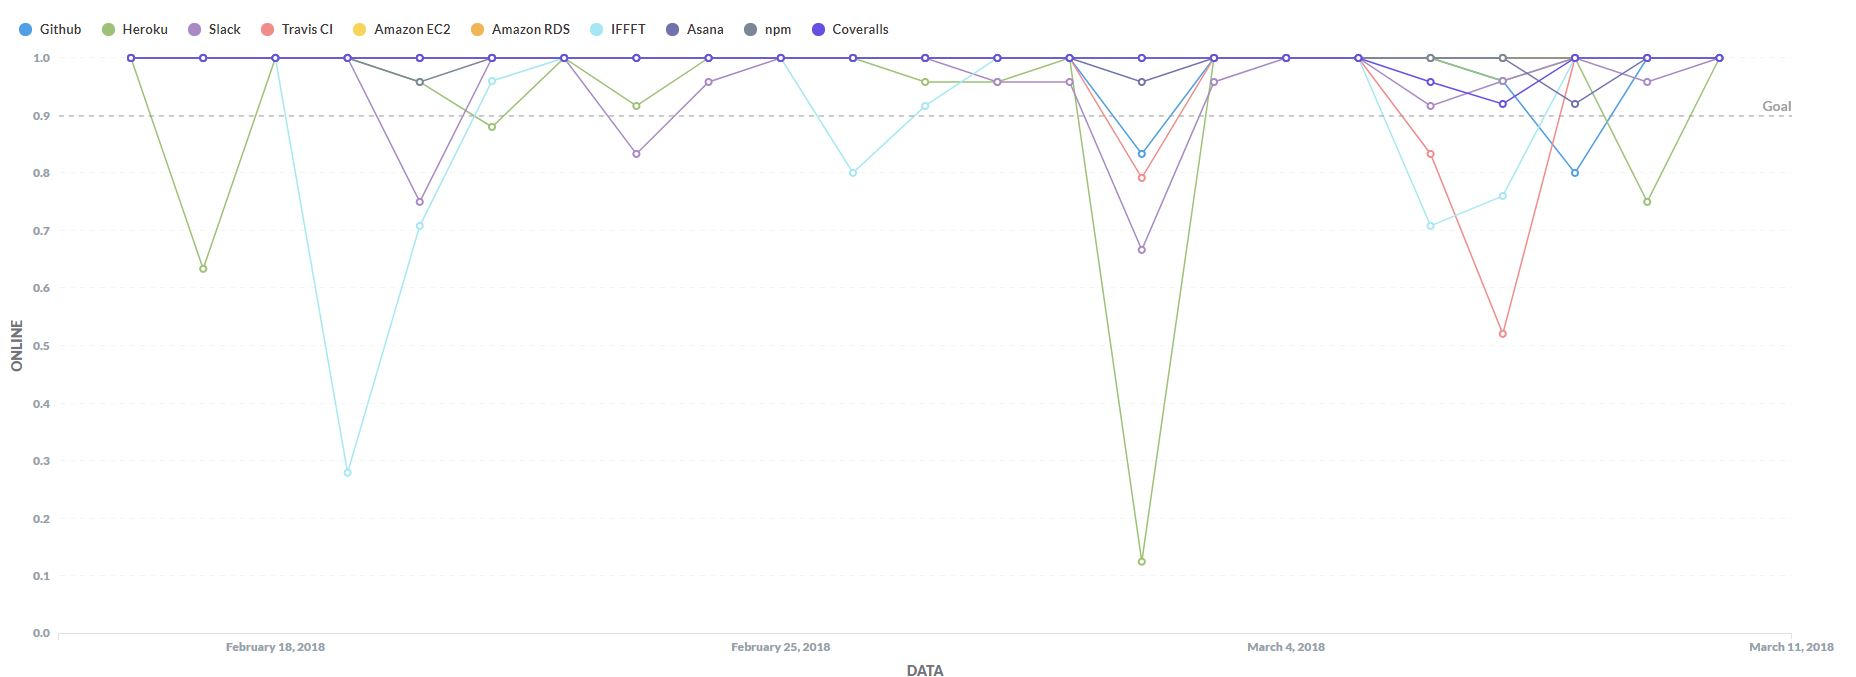
\includegraphics[width=1\linewidth]{RP/MPS007}
	\caption{MPS007}
	\label{fig:processi}
\end{figure}
\\Come si nota dalla figura la maggior parte degli strumenti esterni usati non hanno avuti giornate di indisponibilità.
Solamente Heroku e IFTTT hanno avuto due giornate con un periodo offline del 80/90\% ma essendo strumenti secondari per il lavoro del gruppo non si è ritenuto mettere più di un giorno totale come servizi indisponibili.\\

\textbf{MPS008 Rischi non previsti}\\
Misurazione periodo RP: \textbf{2}
\begin{itemize}
	\item malfunzionamento linea internet \Davide per 3 settimane;
	\item rottura router wifi \Elena per 5 giorni;
\end{itemize}
Due membri del gruppo hanno avuto problemi con l'accesso a internet per lavorare sui documenti e sul prodotto. Sfortunatamente essendo studenti fuori sede non potevano venire a Padova nel periodo del mese di Febbraio, coincidente con la sessione d'esame, hanno però cercato di trovare soluzioni col resto del gruppo scaricando materiale con cui lavorare in modalità offline.

\newpage

\textbf{MPS009 Media commit Github per settimana}\\
Misurazione periodo RP: \textbf{48}
\begin{figure}[htb]
	\centering
	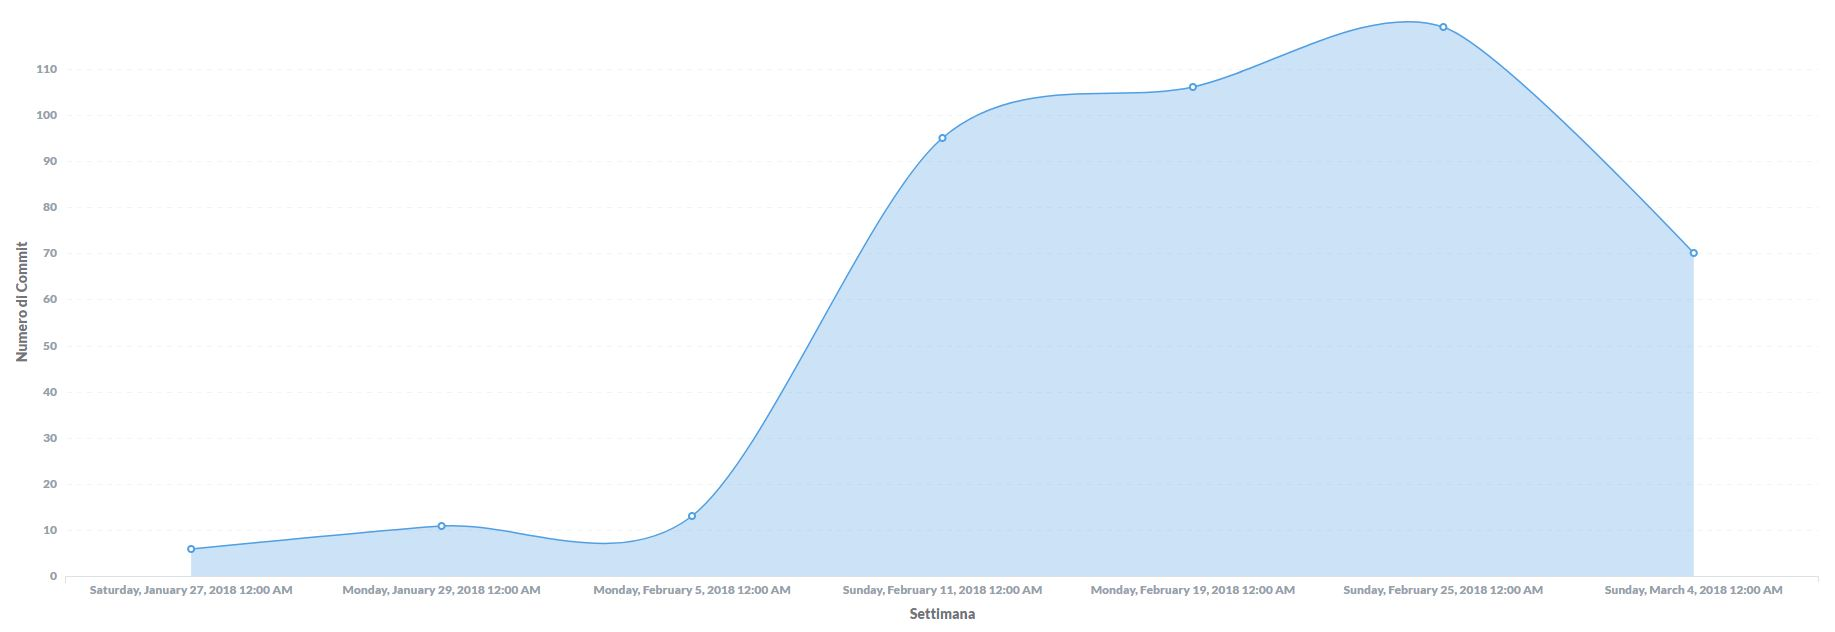
\includegraphics[width=1\linewidth]{RP/MPS009}
	\caption{MPS009}
	\label{fig:processi}
\end{figure}

\textbf{MPS010 Media build Travis per settimana}\\
Misurazione periodo RP: \textbf{60}
\begin{figure}[htb]
	\centering
	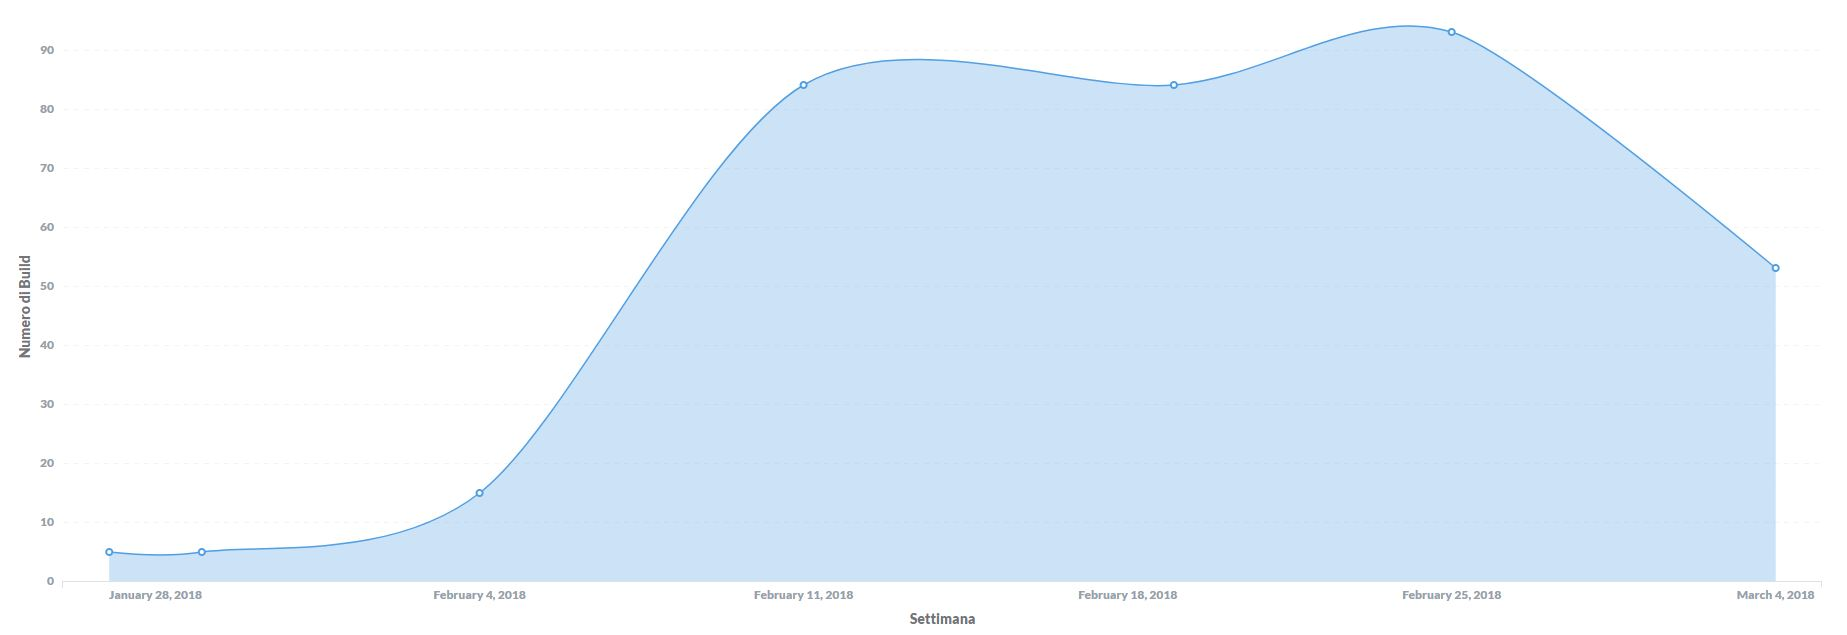
\includegraphics[width=1\linewidth]{RP/MPS010}
	\caption{MPS010}
	\label{fig:processi}
\end{figure}
\\
Come si nota dai precedenti grafici il gruppo ha lavorato costantemente in questo periodo avendo il minor numero di modifiche durante il periodo immediatamente successivo alla pubblicazione dei risultati della Revisione dei Requisiti per dar modo di comprendere le modifiche da effettuare.
Inoltre sempre in questo periodo vi sono stati vari appelli che hanno richiesto molto studio personale da parte dei membri del gruppo.

\newpage

\textbf{MPS011 Percentuale build superate}\\
Misurazione periodo RP: \textbf{77\%}
\begin{figure}[htb]
	\centering
	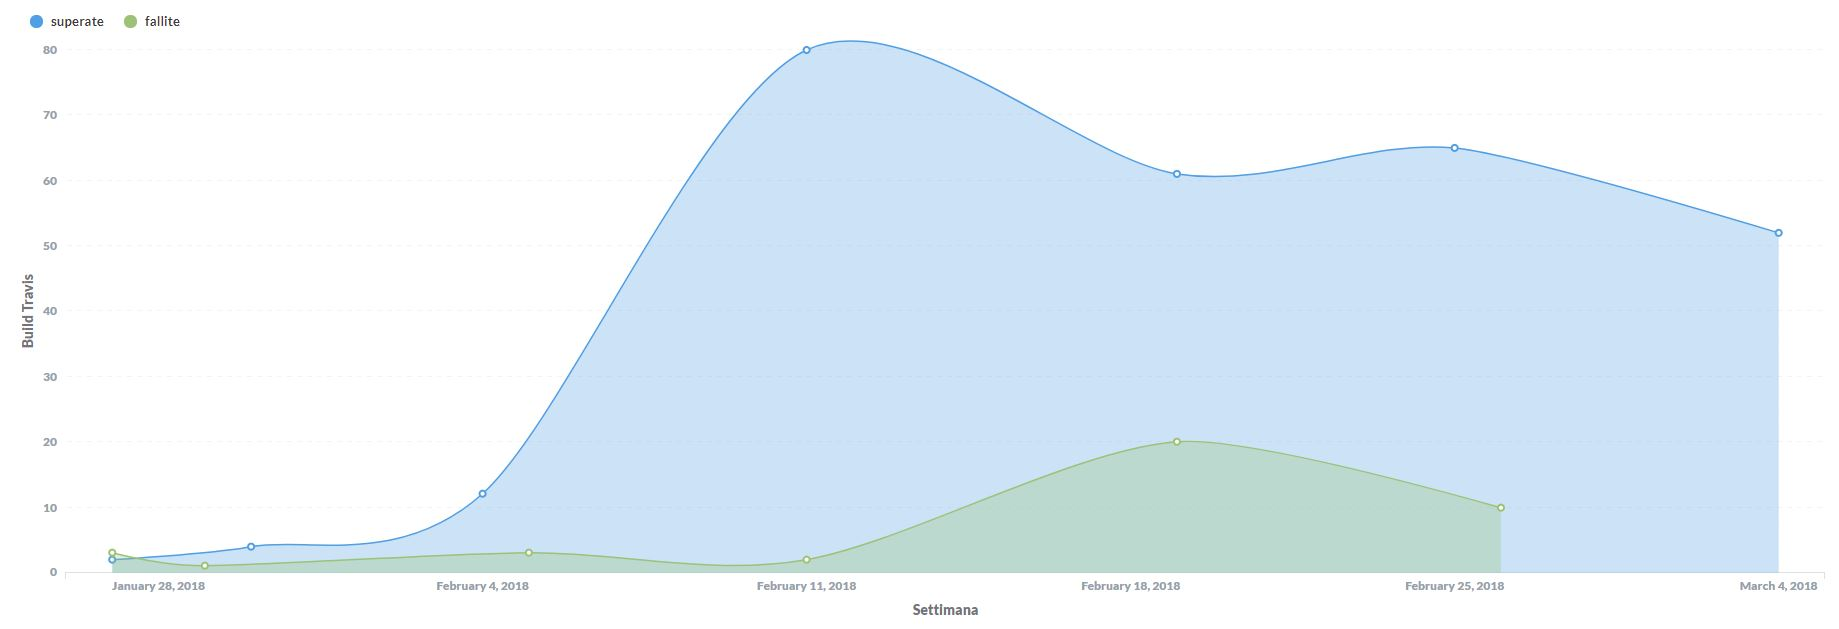
\includegraphics[width=1\linewidth]{RP/MPS011}
	\caption{MPS011}
	\label{fig:processi}
\end{figure}

\subsubsection{Maturità processi ISO 15504}
\begin{figure}[htbp]
	\centering
	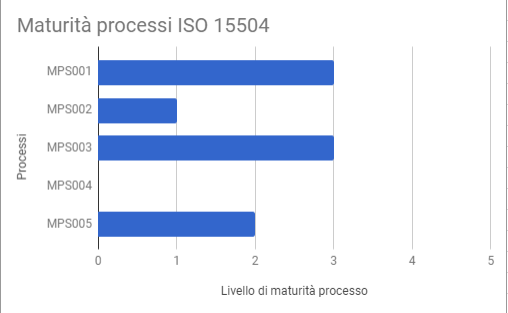
\includegraphics[width=0.7\linewidth]{RP/Processi}
	\caption{Maturità processi}
	\label{fig:processi}
\end{figure}


\newpage
\subsection{Qualità di prodotto}
\subsubsection{Metriche prodotto}
\textbf{MPDD001 Indice di Gulpease}
\begin{figure}[htbp]
	\centering
	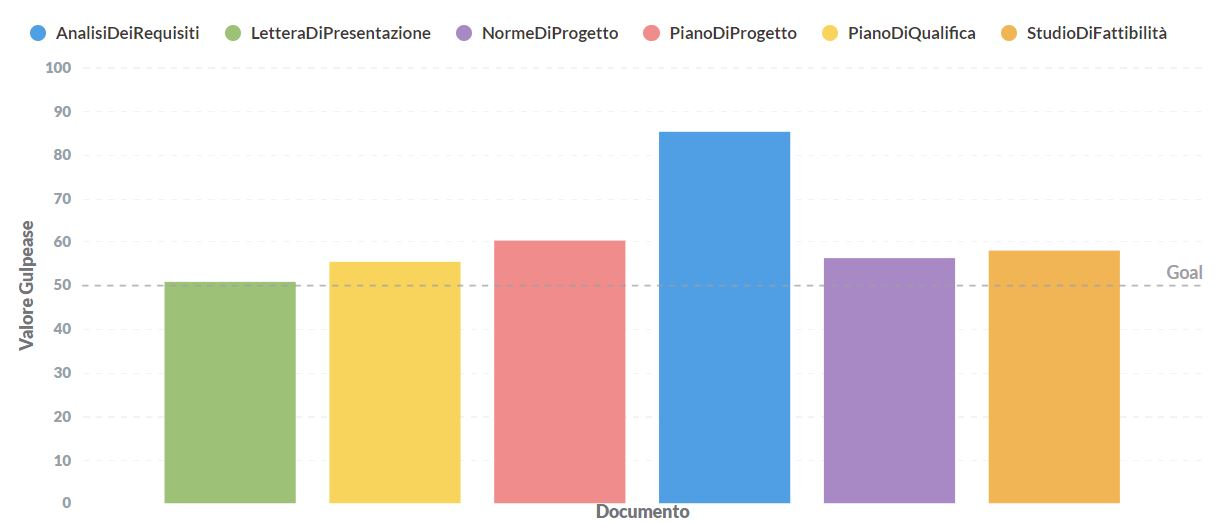
\includegraphics[width=1\linewidth]{RP/gulpease}
	\caption{Ultimo valore Gulpease prima consegna RP}
	\label{fig:processi}
\end{figure}
\begin{figure}[htbp]
	\centering
	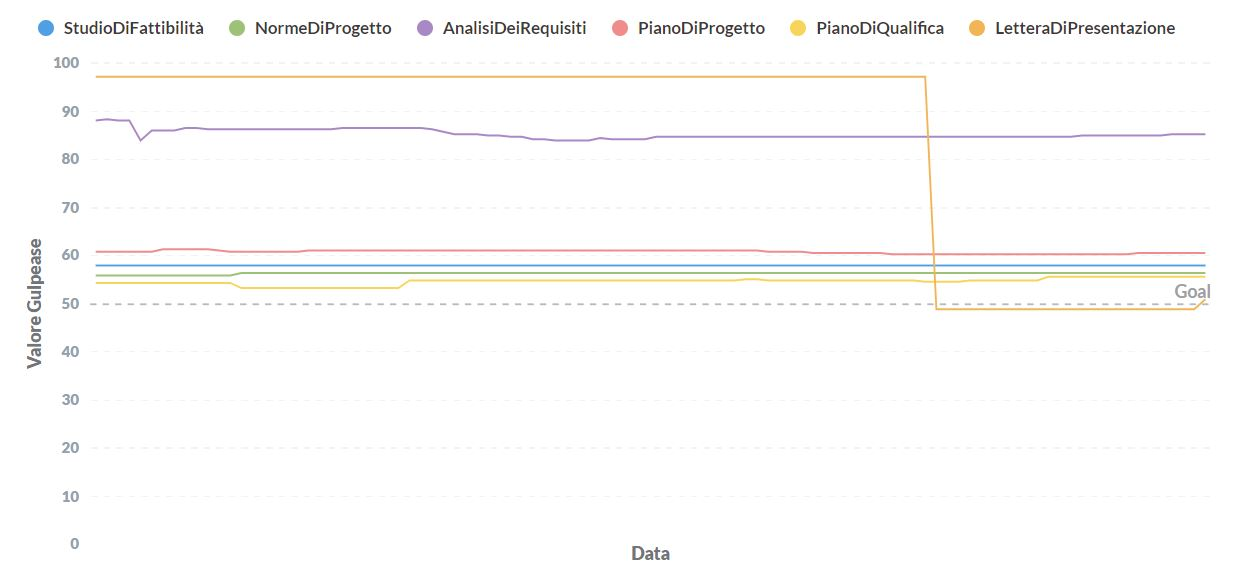
\includegraphics[width=1\linewidth]{RP/gulpeasegrid}
	\caption{Andamento valore Gulpease documenti successivo consegna RR}
	\label{fig:processi}
\end{figure}

\section{Revisione di Qualifica}

\subsection{Qualità di processo}
In questa sezione del documento vengono analizzati i processi, gli esiti delle attività di \citGloss{verifica} svolte su tutti i documenti che vengono consegnati nelle revisioni di progetto e sul prodotto software in sviluppo.

\subsubsection{Metriche processi}

\textbf{MPS001 Schedule Variance}\\
In ogni settimana il valore è rimasto all'interno del range di accettabilità.
\begin{figure}[htb]
	\centering
	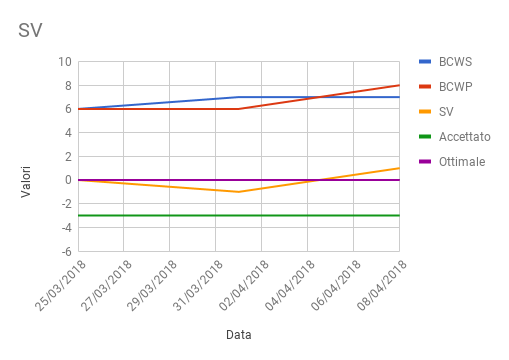
\includegraphics[width=0.7\linewidth]{RQ/SV}
	\caption{MPS001}
	\label{fig:processi}
\end{figure}
\newpage

\textbf{MPS002 Budget Variance}\\
In ogni settimana il valore è rimasto all'interno del range di accettabilità.
\begin{figure}[htb]
	\centering
	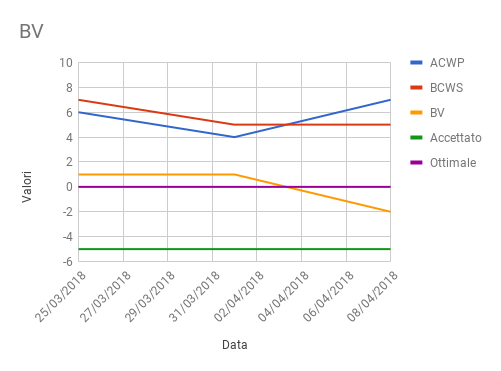
\includegraphics[width=0.8\linewidth]{RQ/BV}
	\caption{MPS002}
	\label{fig:processi}
\end{figure}
\newpage
\textbf{Coverage}
\\
\textbf{MPS003, MPS004, MPS005 e MPS006}
\\\\
\textbf{Solidity Coverage}
\begin{figure}[htb]
	\centering
	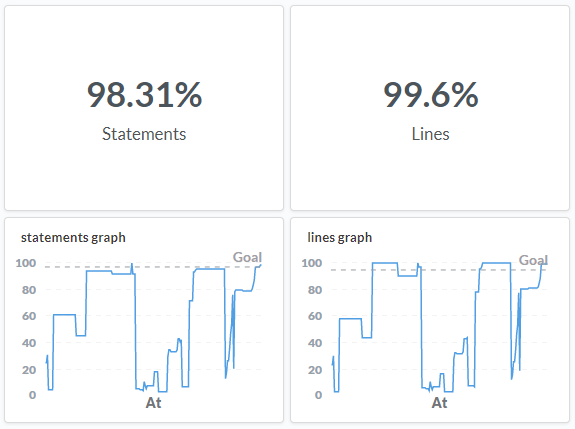
\includegraphics[width=0.8\linewidth]{RQ/SolidityCoverage1}
	\caption{Solidity coverage: statements e lines}
	\label{fig:processi}
\end{figure}
\begin{figure}[htb]
	\centering
	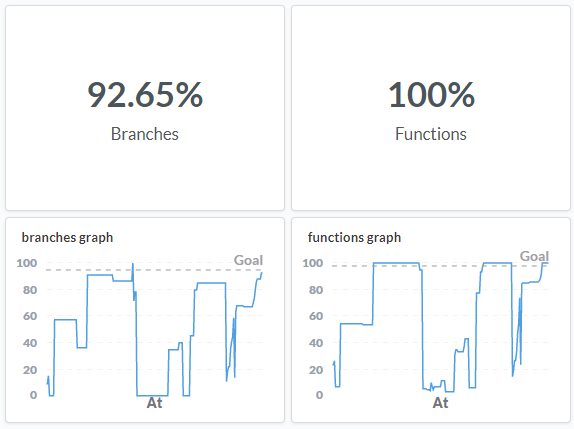
\includegraphics[width=0.7\linewidth]{RQ/SolidityCoverage2}
	\caption{Solidity coverage: branches e functions}
	\label{fig:processi}
\end{figure}
\newpage
\textbf{Javascript Coverage}\\
In questo periodo non è stato avviato il controllo di coverage sulle parti del prodotto scritte in Javascript.\\\\

\textbf{MPS007 Indisponibilità servizi esterni}\\
Misurazione periodo RQ: \textbf{4}
\begin{figure}[htb]
	\centering
	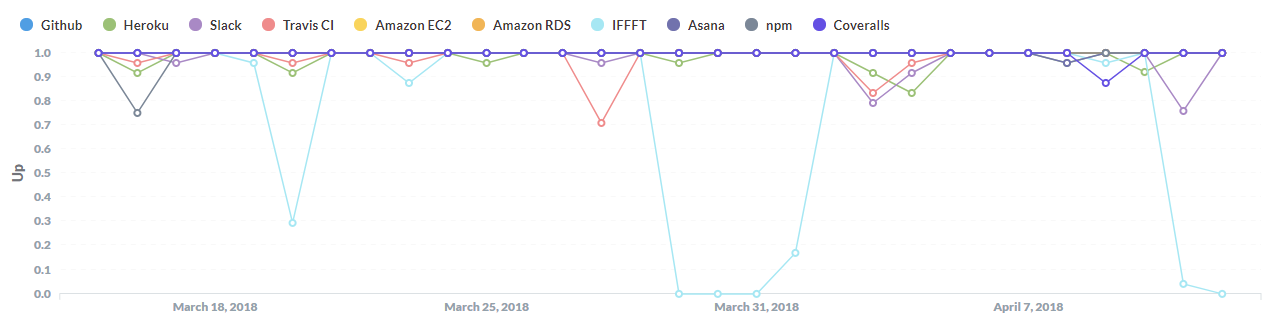
\includegraphics[width=1\linewidth]{RQ/MPS007}
	\caption{MPS007}
	\label{fig:processi}
\end{figure}
\\Come si nota dalla figura la maggior parte degli strumenti esterni usati non hanno avuti giornate di indisponibilità.
Solamente IFTTT è rimasto offline per 4 giorni, ma essendo un servizio secondario allo svolgimento del progetto, non influenza per nulla la sua esecuzione. \\

\textbf{MPS008 Rischi non previsti}\\
Misurazione periodo RQ: \textbf{0}\\
In questo periodo non è incorso nessun rischio imprevisto.\\


\textbf{MPS009 Media commit Github per settimana}\\
Misurazione periodo RQ: \textbf{56}
\begin{figure}[htb]
	\centering
	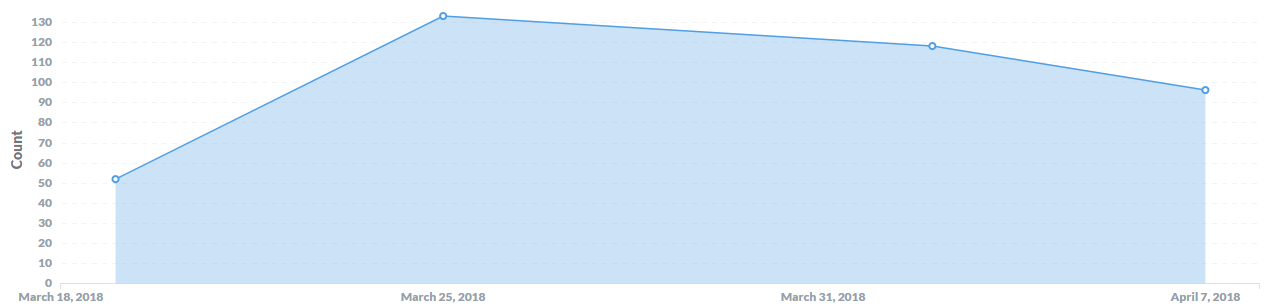
\includegraphics[width=1\linewidth]{RQ/MPS009}
	\caption{MPS009}
	\label{fig:processi}
\end{figure}
\\

\textbf{MPS010 Media build Travis per settimana}\\
Misurazione periodo RQ: \textbf{50}
\begin{figure}[htb]
	\centering
	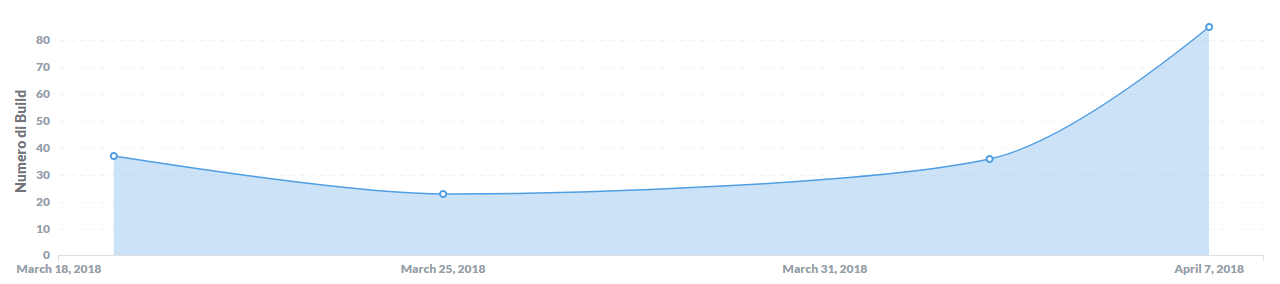
\includegraphics[width=1\linewidth]{RQ/MPS010}
	\caption{MPS010}
	\label{fig:processi}
\end{figure}
\\
Nel periodo centrale il numero di build è stato minore del resto perché ci si è focalizzati sulla progettazione dell'architettura del prodotto e della creazione dei corrispettivi diagrammi UML.

\newpage
\textbf{MPS011 Percentuale build superate}\\
Misurazione periodo RQ: \textbf{76\%}
\begin{figure}[htb]
	\centering
	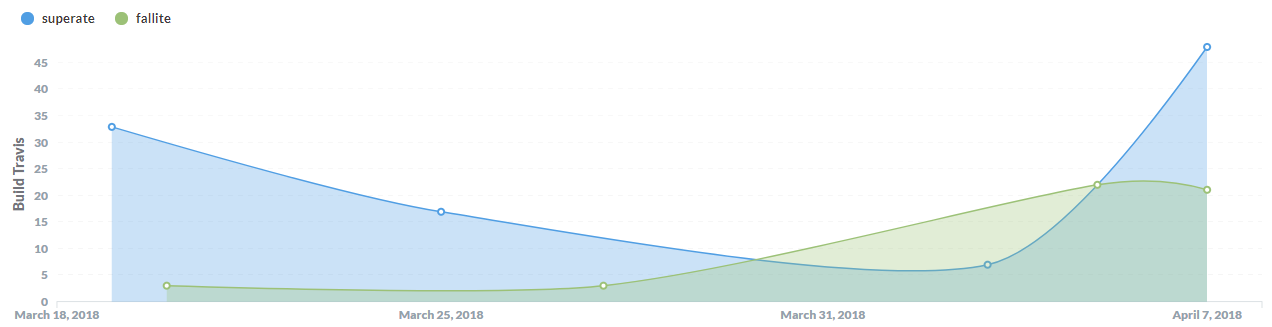
\includegraphics[width=1\linewidth]{RQ/MPS011}
	\caption{MPS011}
	\label{fig:processi}
\end{figure}

\subsubsection{Maturità processi ISO 15504}
\begin{figure}[htbp]
	\centering
	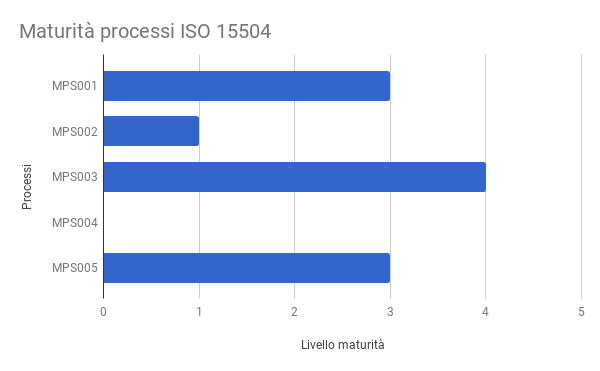
\includegraphics[width=0.7\linewidth]{RQ/Processi}
	\caption{Maturità processi}
	\label{fig:processi}
\end{figure}


\newpage
\subsection{Qualità di prodotto}

\subsubsection{Metriche prodotto}

\textbf{MPDD001 Indice di Gulpease}
\begin{figure}[htbp]
	\centering
	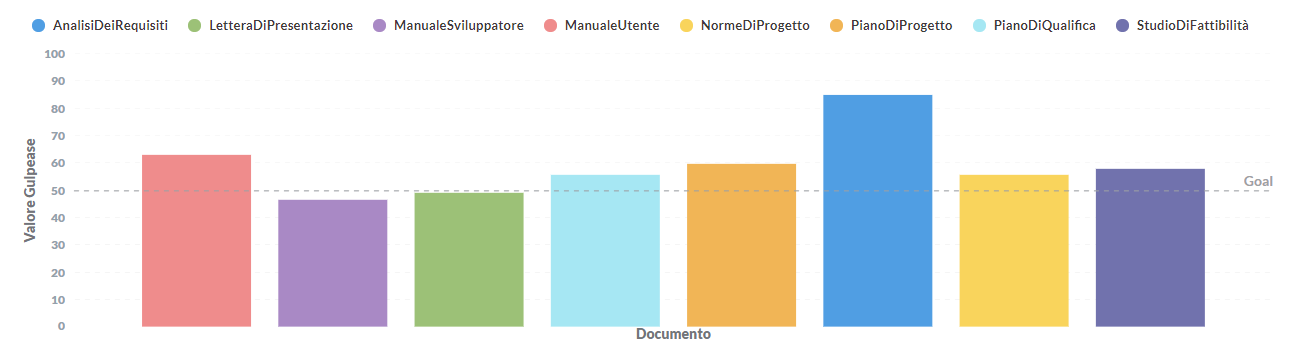
\includegraphics[width=1\linewidth]{RQ/gulpease}
	\caption{Ultimo valore Gulpease prima consegna RQ}
	\label{fig:processi}
\end{figure}

\textbf{MPDD002 Indice di Flesch}
\begin{figure}[htbp]
	\centering
	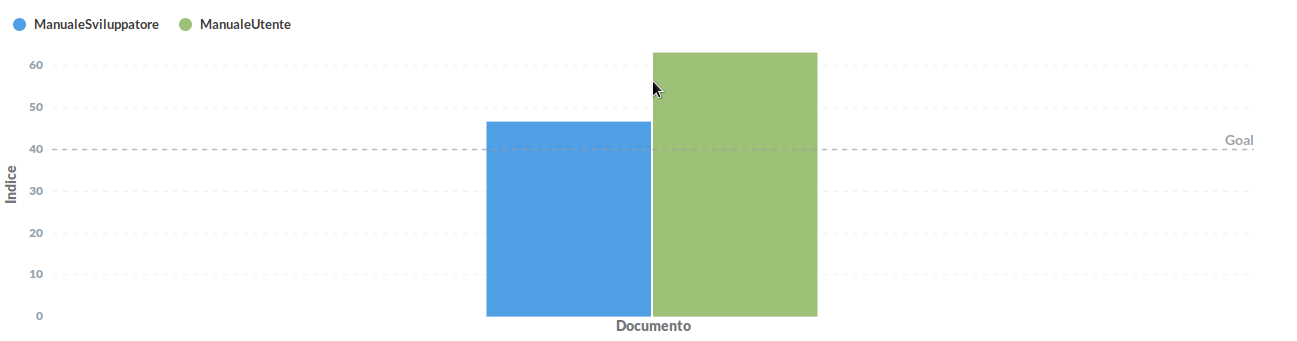
\includegraphics[width=1\linewidth]{RQ/flesch}
	\caption{Ultimo valore Flesch prima consegna RQ}
	\label{fig:processi}
\end{figure}

\begin{figure}[htbp]
	\centering
	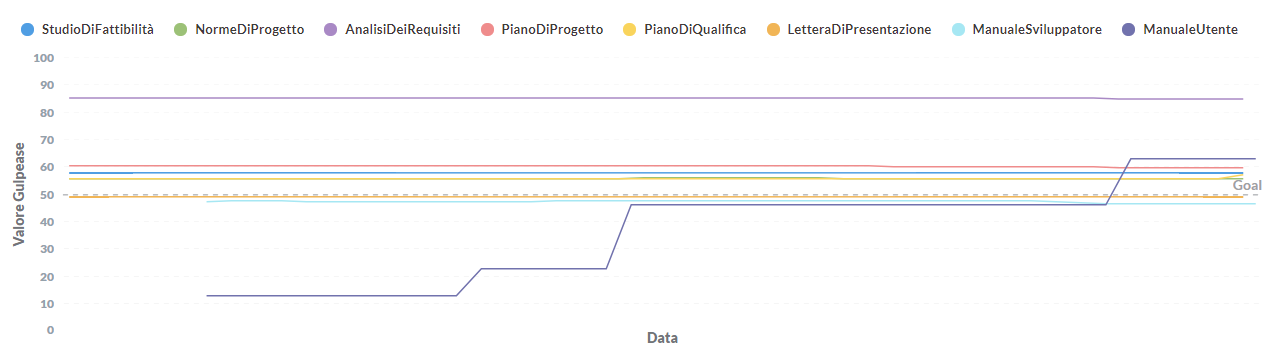
\includegraphics[width=1\linewidth]{RQ/gulpeasegrid}
	\caption{Andamento valore Gulpease documenti successivo consegna RP}
	\label{fig:processi}
\end{figure}

\section{Revisione di Accettazione}
Questa sezione verrà implementata alla fine del periodo indicato.

\end{document}